\section{Native Self-Evolution and Composable Recipes}
\label{sec:recipes}

\subsection{Native: goal-aware, viability-gated self-evolution}
\label{sec:native}

% Role: motivation. Message: a supplied measurement need not exhaust the objective.
Native studies self-evolution when the objective is not necessarily identical to an external score. A natural-language goal can be fully operationalized by a benchmark, or only partly measured by it. The default protocol asks the harness to judge that relationship and to add or revise its own tests when useful. It does not mandate extra tests or treat a self-reported score as an independent measurement. The legacy interface also permits a goal without an evaluator, or open-ended exploration without a supplied goal; those are explicit settings rather than evidence of autonomous capability growth.

% Role: method. Message: the running harness proposes changes to its own declared state.
The reference episode uses \emph{observe, propose, act, reflect}. The active harness inspects its state and permitted evidence, chooses a scoped change, edits its pending candidate, and records outcomes and unresolved risks. The four phase names alone are not the contribution. The relevant experimental choices are which goal and evidence are supplied, what state the harness can change, which implementation executes each phase, and how a candidate becomes active. For supported staged-source adapters, all phases run the frozen last-valid source, including reflection; pending edits take effect only after validation and activation. Self-authored tests remain part of the harness state, distinct from the external grader.

% Role: formalization. Message: the common profile has an explicit non-score admission rule.
The common-contract profile separates the active harness $A_t$ from the working candidate $W_t$. For an episode that completes successfully and publishes a candidate, let it produce $\widetilde W_{t+1}=F_\theta(A_t,W_t,G,V_t)$, where $G$ is the supplied goal, $V_t$ is permitted evidence, and the model weights $\theta$ remain fixed. With a model-free viability check $v$, its transition is
\begin{equation}
 W_{t+1}=\widetilde W_{t+1},\qquad
 A_{t+1}=\begin{cases}
 \widetilde W_{t+1}, & v(\widetilde W_{t+1})=1,\\
 A_t, & v(\widetilde W_{t+1})=0.
 \end{cases}
\label{eq:native-transition}
\end{equation}
There is no condition requiring an external score to increase. A viable candidate becomes active even if its measured task score decreases; an invalid candidate remains the exact working state for a later repair episode while execution retains $A_t$. An actor/stage failure or an uncertain external operation stops this transition and follows the shared failure/recovery protocol; it is not silently treated as a viability rejection. This defines a continuation policy, not a monotonic-improvement guarantee. The final candidate is the last valid one, not an outer-loop score maximum.

\begin{figure}[t]
\centering
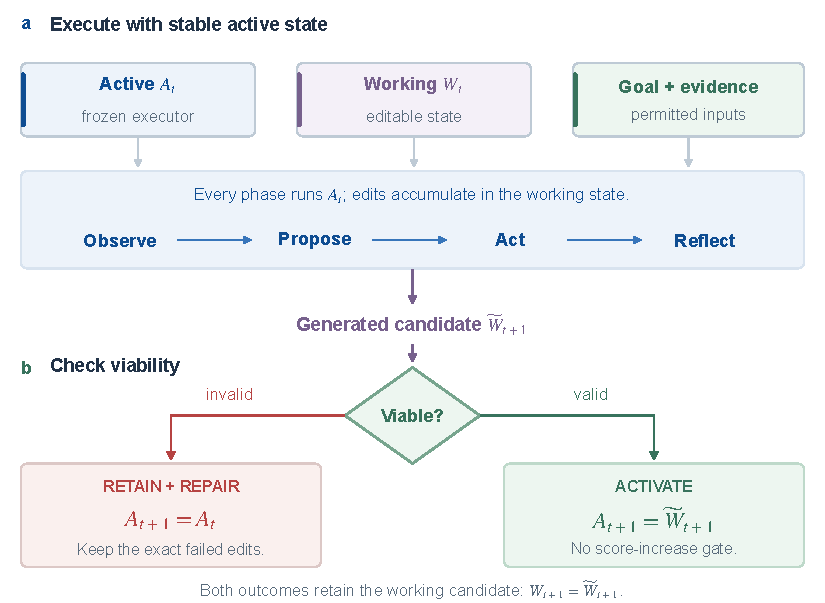
\includegraphics[width=\linewidth]{figures/native-transition.pdf}
\caption{\textbf{Native common-profile transition.} The current active harness executes the episode while changes accumulate in a separate working candidate. A source-bound viability result controls activation. Completed but nonviable edits remain available for repair, and formal scores enter later reasoning only through the declared evidence policy; they do not implement an outer acceptance filter. This figure describes supported staged-source execution, not every legacy adapter's lifecycle.}
\label{fig:native}
\end{figure}

% Role: scope. Message: the two Native profiles must not be conflated.
The common profile requires observed evaluation pools, evaluates the initial and each viable candidate, and runs optional hidden tests after evolution. It binds evolution and subject roles to the same harness integration and uses exactly one managed episode stage. Its supported phase controls do not make it an arbitrary stage graph. Legacy Native retains its separate goal/no-goal options, evaluator schedules, dispositions, measurements, and selection settings. Accordingly, the no-outer-score rule in Equation~\ref{eq:native-transition} describes the common profile; it must not be generalized to every legacy configuration.

% Role: evidence and limitation. Message: current evidence supports the mechanism, not its advantage.
The source-bound Native fixture demonstrates invalid-edit retention, later repair, changed candidate execution, private final grading, and replay. Bounded Pi/DSH pilots additionally exercise one common episode; the broader engineering record tests supported source activation paths. These support the implemented state transition. They do not establish that goal-aware self-evolution beats score-guided search, that self-authored tests are useful, or that useful improvements compound. Such claims require matched comparisons varying objective framing, evidence access, activation/selection policy, and self-evidence while holding tasks, models, initial artifacts, and budgets fixed.


\subsection{Reference recipes and researcher workflow}

% Role: overview. Message: recipe reuse preserves method semantics.
The included recipes demonstrate several ways to reuse infrastructure without equating their algorithms. Table~\ref{tab:profiles} identifies the optimized artifact, controlling mechanism, and empirical boundary of each family. The method documentation and frozen profile configurations specify the actual options; family names alone are insufficient to reconstruct an experiment. In particular, an original-domain builder is an entry point for preparing a new study, not a certificate that the resulting configuration has model-quality evidence.

\begin{table}[t]
\caption{Implemented profile boundaries. Reuse is explicit at the artifact, stage, or service layer. A family name is not a claim of all upstream options or matched-paper results.}
\label{tab:profiles}
\small
\begin{tabularx}{\linewidth}{@{}>{\raggedright\arraybackslash}p{0.14\linewidth}>{\raggedright\arraybackslash}p{0.17\linewidth}Y Y@{}}
\toprule
Family & Candidate & Included mechanism & Evidence boundary \\
\midrule
GEPA & Text components & Single-mutation loop, instance frontier, round-robin components & Adapted AIME study; no merge/cache in this profile. \\
ACE & Structured playbook & Generator, reflector, curator; incremental updates; offline/online & Adapted Formula studies; online stream differs from final held-out scoring. \\
Meta-Harness & Memory-system code & Historical evidence retrieval, proposal workspace, learning and selection & Historical JSON proposer; actual coding proposers have bounded pilots. \\
Combee & Base-method artifact & ACE/GEPA aggregation, parallel maps and fixed/dynamic batches & Formula results and separate model-free common trace; no isolated speedup. \\
CORAL & Program and shared knowledge & Worker generations, formal submissions, sourced knowledge, event policies & Adapted circle packing; separate three-request directed qualification. \\
Native & Harness source/state & Legacy compatibility; additional common-stage evolution profile & Source activation/repair and external evaluation; no universal Native phase requirement. \\
\bottomrule
\end{tabularx}
\end{table}


% Role: example. Message: ACE and Combee compose at a real reusable boundary.
\paragraph{ACE with Combee.}
ACE's generator, reflector, and curator operate on a versioned playbook whose structured updates retain stable entries and counters. Combee-ACE reuses that representation and the surrounding evaluation services, while introducing grouped parallel proposal work and aggregation before publication. The implementation distinguishes original samples from copied aggregation occurrences and preserves their provenance. Sequential ACE, naive parallel, fixed Combee, and dynamic Combee therefore form explicit conditions rather than informal choices of thread count. The common frozen-trace check in Section~\ref{sec:mechanism} isolates these consumption and update mechanisms.

% Role: example. Message: GEPA and Combee compose without replacing the search loop.
\paragraph{GEPA with Combee.}
Combee aggregation is also integrated into the pinned GEPA search loop. GEPA retains candidate evaluation, acceptance, component choice, and final testing, while the aggregation operator changes how reflective proposals are formed. This is a second implemented composition, with its own artifact and parser requirements. The existence of both integrations supports component reuse across base learners; it does not establish that a Combee operator can be attached to any method without adapting its input and update contracts. The historical Formula results in this report concern Combee-ACE, not a new Combee-GEPA benchmark.

% Role: example. Message: a self-evaluator is an explicit experiment intervention.
\paragraph{An explicit self-evaluation experiment.}
A stage-composing method can insert a self-evaluator between a proposal and the next method decision. The researcher declares its inputs, the permitted evidence view, the output type, and whether that output affects revision, selection, or only logging. An ablation can then remove or replace the stage while keeping tasks, external grading, budgets, and other choices fixed. The tutorial demonstrates such configuration and plugin boundaries. It supplies a way to pose the research question; a useful or calibrated self-evaluator would still require independent empirical validation.

% Role: example and boundary. Message: Native is one implementation, with two paths.
\paragraph{Native evolution as a method.}
The legacy Native compatibility recipe preserves the existing episode transaction engine and its evaluator schedules and measurements. The additional common Native evolution profile uses ordinary stages, immutable candidates, shared evaluation, and the recovery journal while retaining observe/propose/act/reflect inside its episode stage. It uses neutral disposition and last-valid activation, not outer-score selection. The same integration supplies its evolution and target roles. These paths are documented separately; neither is imposed on ACE, GEPA, Meta-Harness, Combee, or CORAL.

% Role: workflow. Message: configure existing behavior, extend missing behavior.
\paragraph{From an experiment idea to a run.}
The normal workflow is to choose a profile, bind compatible actors and artifacts, declare tasks and evidence policy, then validate and lock sources before running. Replacing an implemented model, prompt, policy, budget, or exposed stage is a configuration change. Introducing a new update rule, actor protocol, or side effect requires the corresponding plugin and its checks. Resume uses the original locks; a changed method or runtime creates a new experiment. Thus, ``no model training'' is not sufficient for configuration-only reproduction of an arbitrary new method.

% Role: ecosystem. Message: skills provide guidance rather than performance.
\paragraph{Agent-facing use and contribution skills.}
The accompanying documentation commit includes a \code{proteus-use} skill that guides an agent through profile choice, role binding, validation, execution or saved-run analysis, recovery, and reporting. An optional \code{proteus-contribute} skill guides extension work. These repository-distributed instructions reference the matching runtime and documentation, distinguish an analysis-only request from a new experiment, and keep evidence and resource limits explicit. They are a usability and contribution interface, not an additional optimizer or a demonstrated performance contribution. Their committed documentation provenance is recorded separately from the source revisions that produced the experimental evidence.
